\section{Replacements of pixels.}
\begin{enumerate}[label=\emph{\alph*)}]
\item Let us call the monochrome image from your answer to the last item of the previous question A , and the other one B . Take the center square region of $100 \times 100$ pixels of A and insert it into the center of B.

The results are shown in figure \ref{fig:replace-center}.
\begin{figure}[h!]
\centering
\begin{subfigure}{0.5\textwidth}
  \centering
  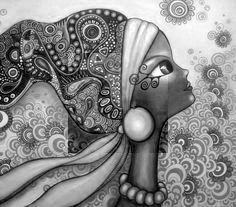
\includegraphics[width=0.5\linewidth]{../output/p0-3-a-0.jpg}
  \caption{Output for the input p0-1-0.jpg}
  \label{fig:sfig1}
\end{subfigure}%
\begin{subfigure}{0.5\textwidth}
  \centering
  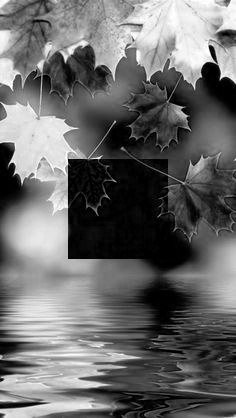
\includegraphics[width=0.5\linewidth]{../output/p0-3-a-1.jpg}
  \caption{Output for the input p0-1-1.jpg}
  \label{fig:sfig2}
\end{subfigure}
\begin{subfigure}{0.5\textwidth}
  \centering
  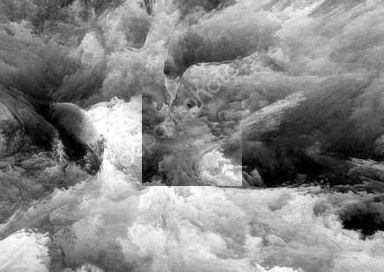
\includegraphics[width=0.5\linewidth]{../output/p0-3-a-2.jpg}
  \caption{Output for the input p0-1-2.jpg}
  \label{fig:sfig1}
\end{subfigure}%
\begin{subfigure}{0.5\textwidth}
  \centering
  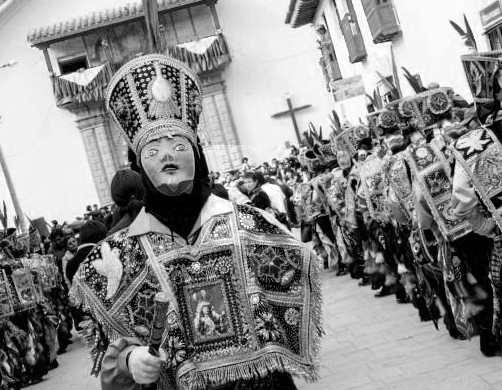
\includegraphics[width=0.5\linewidth]{../output/p0-3-a-3.jpg}
  \caption{Output for the input p0-1-3.jpg}
  \label{fig:sfig2}
\end{subfigure}
\caption{Output images for question 3.a}
\label{fig:replace-center}
\end{figure}

\item Replace the respective channel of B into the original image.

The results are shown in figure \ref{fig:replace-channel}.

\begin{figure}[h!]
\centering
\begin{subfigure}{0.5\textwidth}
  \centering
  
\includegraphics[width=0.5\linewidth]{../output/p0-3-b-0.jpg}
  \caption{Output for the input p0-1-0.jpg}
  \label{fig:sfig1}
\end{subfigure}%
\begin{subfigure}{0.5\textwidth}
  \centering
  
\includegraphics[width=0.5\linewidth]{../output/p0-3-b-1.jpg}
  \caption{Output for the input p0-1-1.jpg}
  \label{fig:sfig2}
\end{subfigure}
\begin{subfigure}{0.5\textwidth}
  \centering
  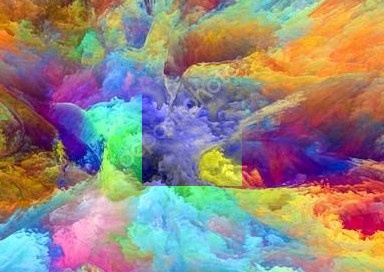
\includegraphics[width=0.5\linewidth]{../output/p0-3-b-2.jpg}
  \caption{Output for the input p0-1-2.jpg}
  \label{fig:sfig1}
\end{subfigure}%
\begin{subfigure}{0.5\textwidth}
  \centering
  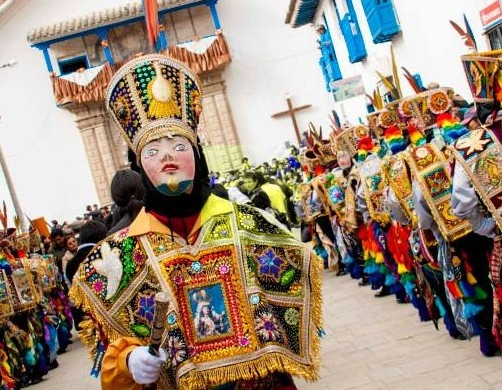
\includegraphics[width=0.5\linewidth]{../output/p0-3-b-3.jpg}
  \caption{Output for the input p0-1-3.jpg}
  \label{fig:sfig2}
\end{subfigure}
\caption{Output images for question 3.b}
\label{fig:replace-channel}
\end{figure}

In 3.a the differences are easier to see in the images \ref{fig:replace-center}.a, \ref{fig:replace-center}.c, in the same occurs in 3.b. This happens because these images presents higher green than red values in its center areas, generating more purple-blue colors which is reflected as darker points in the monochromatic image. In the images \ref{fig:replace-center}.b,  \ref{fig:replace-center}.d, the red colors turn to yellow which is lighter in the monochromatic image.

\end{enumerate}
